\chapter{Implementation}

The goal of this thesis is to combine the advantages of passive and active capacity estimation tools and possibly eliminate their flaws in an attempt to get as accurate estimation results as possible.

We have set the requirements that should be met in order to consider our goal achieved:\\
Firstly, the tool should minimize the intrusion into the network we are trying to measure.\\
Secondly, the tool must deliver the accurate results despite the obstacles and challenges it might have to face during measurements, such as flow interference.


\section{Approach}
The basic idea of the proposed methodology is to send multiple TCP packets from the source host to the destination host and measure the capacity of the path to each router that the generated packets pass.
\\Every packet sent from the source has the \texttt{time to live} value adjusted in a way that it expires when the packet reaches the targeted router. 
\\As a consequence each router generates ICMP time exceeded messages and sends them back to the original sender. The captured inter-arrival times are then passed to the PPrate algorithm and it calculates the capacity from the Sender host to each router respectively. 

\begin{figure}[h]
 \centering
 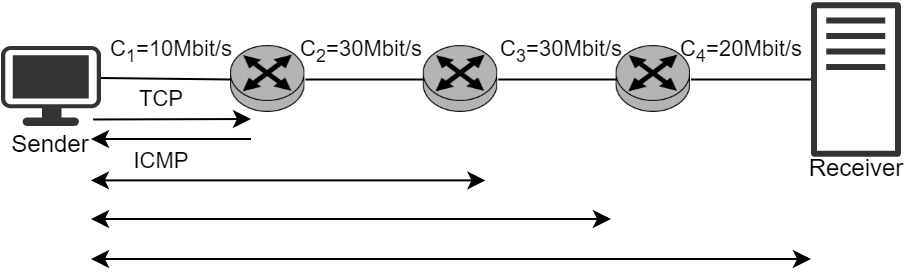
\includegraphics[width=\textwidth]{approach}
 \caption{The basic idea of the capacity estimation method}
 \label{approach}
\end{figure}

The first router with the smallest capacity will be the end of the bottleneck link.
To be more specific, our method does not guarantee to estimate the exact capacity of each link, rather the capacity of the path from the source to each router.
For example, in the figure \ref{approach} where a sample topology is depicted, the first link is the narrow one. Our method will return the capacity of 10 for each hop instead of the original 30, 30 and 20 respectively. This also serves as an indication on the location of the narrow link.\\
Moreover, if there are multiple narrow links on the path, our tool in only able to locate the first one.

In order to calculate the capacity of the last link, we incorporate Brzoza's\cite{Brzoza} framework into our program, which estimates capacity end-to-end. This is necessary in order to find out whether the last hop is the narrowest link or not.\\

\begin{figure}[h!]
 \centering
 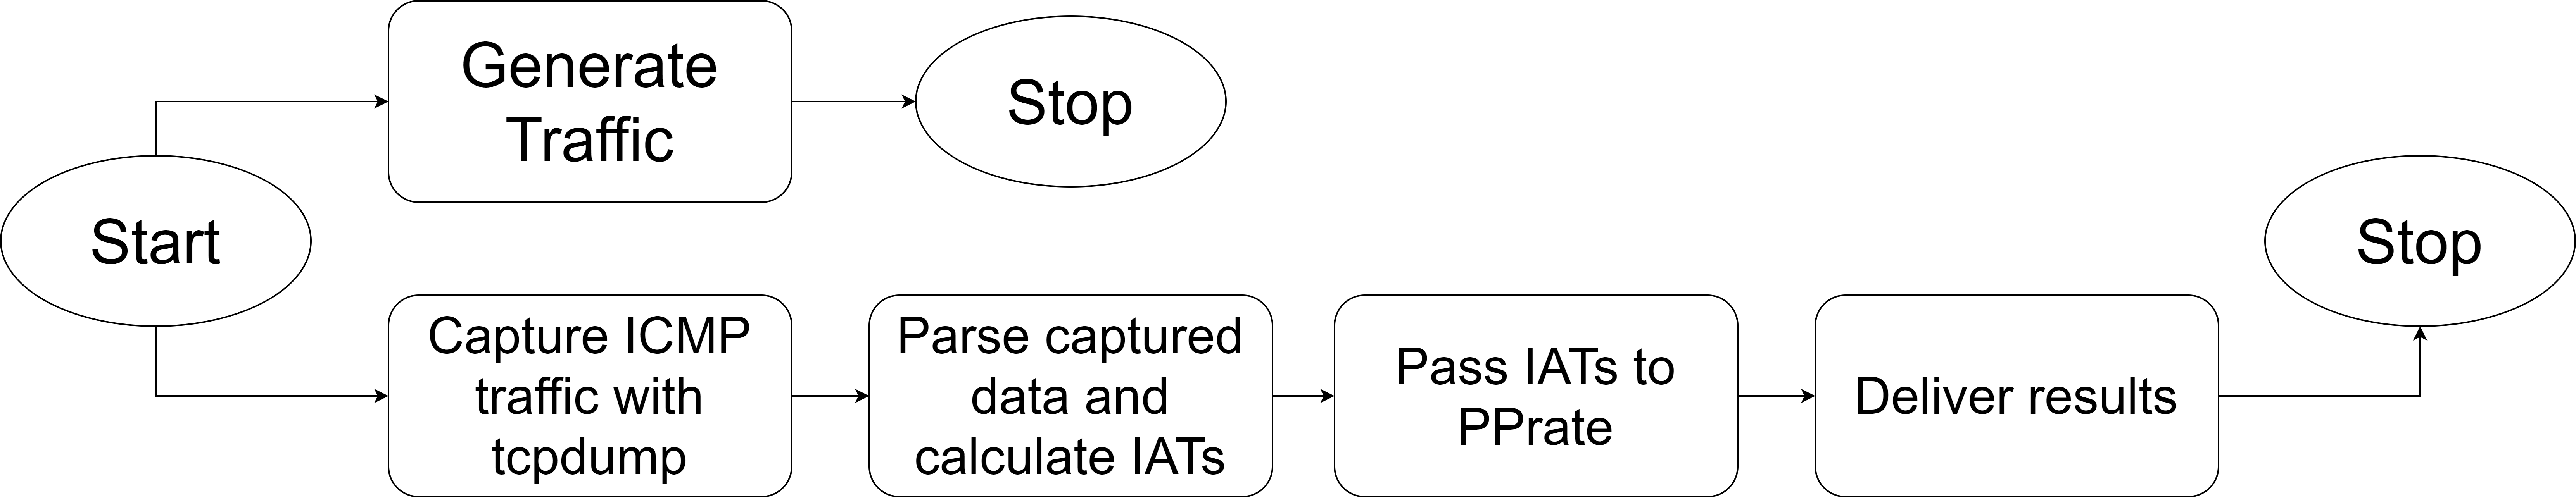
\includegraphics[width=\textwidth]{flowchart2}
 \caption{Flow of the capacity estimation tool}
 \label{flowchart}
\end{figure}


The basic flow of our approach as shown in the figure \ref{flowchart} is executed as follows:
\begin{itemize}
  \item The tool generates TCP packets and sends them through the path directed to the destination host via raw sockets. Each packet has a time-to-live value adjusted the way that they expire at the targeted router so that ICMP messages are generated and sent back to the source.
  \item In parallel \texttt{tcpdump}\cite{tcpdump_man} command is listening and capturing all the ICMP packets that return to the sender host. 
  \item We aim a configurable amount of packets at each router and once the traffic generator covers all the hops on the path, it stops.
  \item After capturing all the ICMP time exceeded packets the program parses them and calculates inter-arrival times separately for each hop.
  \item These inter-arrival times are then passed to the PPrate algorithm which calculates the capacities from the host to each router on the path.
\end{itemize}

As this thesis builds upon the work by P. Brzoza\cite{Brzoza} and uses his PPrate implementation in Python, as well as other important parts of his work, we also find it reasonable and more importantly practical to also implement our work in Python, which in turn is a very powerful tool to work with data analysis. Additionally, we implement the traffic generation part in \texttt{C} programming language as it provides the ability to manually build data packets via raw sockets.

\section{Traffic Generation}
\label{traffic_gen}
In this section we will briefly explain how the traffic generation works in our tool.

We use raw sockets because they enable to manually build a packet and therefore also configure an IP header of the packet. 
\begin{lstlisting}[caption={Creation of a packet\cite{tcp_raw_sockets}}, language=C, showstringspaces=false]
// Creating a packet
char packet[4096] , source_ip[32] , *data , *pseudogram;

//zero out the packet buffer
memset (packet, 0, 4096);

//IP header
struct iphdr *iph = (struct iphdr *) packet;

//TCP header
struct tcphdr *tcph = (struct tcphdr *) (packet + sizeof (struct ip));
struct sockaddr_in sin;
struct pseudo_header psh;

//Data part
data = packet + sizeof(struct iphdr) + sizeof(struct tcphdr);
\end{lstlisting}

As mentioned in section \ref{ip_descr}, the IP header contains a field \texttt{Time to live (TTL)}, which has to be controlled by the sender so that it can target each router on the path. Therefore, we first assign the value of 1 to the \texttt{iph->ttl} field in order to get the ICMP responses from the first router. 

\begin{lstlisting}[language=C, showstringspaces=false]
iph->ttl = 1; 
\end{lstlisting}

Finally, the tool generates the traffic with a \texttt{while} loop. 
Depending on the desired packet train length \texttt{iph->ttl} is being incremented after the specific amount \texttt{n}, which denotes the train length and then targets the next router on the path until it reaches the final host.\\
The traffic is terminated once the  \texttt{iph->ttl} surpasses the number of hops on the path. 

\begin{lstlisting}[caption={Generating traffic towards the destination host}, language=C, showstringspaces=false, breaklines=true]
int i = 0;
while (1)
{
    //Send the packet
    if (sendto(s, packet, iph->tot_len, 0, (struct sockaddr *) &sin, sizeof(sin)) < 0)
    {
        perror("sendto failed");
    }
    //Data sent successfully
    else
    {
        printf("%d \t", i+1);
        printf ("Packet Sent. Length: %d \n", iph->tot_len);
    }
    
    // ttl should be incremented after every n packets
    i++;
    if(i == n) // number of packets necessary for measuring
    {
        printf("hop #%d done\n\n", iph->ttl);
        iph->ttl++;
        i = 0;
    }
    
    if(iph->ttl == routers+2) // total number of routers + 2
    {
        break;
    }
}
\end{lstlisting}


\section{Capturing the Traffic and Estimating Capacities}

The whole process described in the section \ref{traffic_gen} is executed in parallel with the \texttt{tcpdump} command which serves as an ICMP listener and captures every ICMP packet generated by the routers. For that we need to adjust \texttt{tcpdump} so that it can filter every other type of traffic with the following script:

\begin{lstlisting}[language=bash]
tcpdump -n icmp -w results/icmp.pcap
\end{lstlisting}

Additionally, we execute another \texttt{tcpdump} to capture the TCP traffic separately for end-to-end capacity estimation:

\begin{lstlisting}[language=bash]
tcpdump -n tcp -w results/tcp.pcap
\end{lstlisting}

The captured data is subsequently converted to \texttt{.csv} format with the following \texttt{tshark} command:

\begin{lstlisting}[language=bash, breaklines=true]
tshark -r results/icmp.pcap -T fields -E header=y -E separator=, -E quote=d -E occurrence=f -e frame.time_epoch -e ip.src -e ip.dst -e ip.len > results/icmp.csv 
\end{lstlisting}

Finally we extract the arrival times of the ICMP packets grouped by routers that have generated them, calculate the inter-arrival times and pass the lists of IATs to PPrate:

\begin{lstlisting}[caption={Calculating capacities hop-by-hop with PPrate\cite{Brzoza}}, language=Python]
def calculate_capacities():
    pcap_to_csv()
    filepath = dir_path + "/results/icmp.csv"
    streams = {}

    df = read_from_csv(filepath)
    packet_size = get_packet_size()
    group_by_routers(df, streams)
    results = []
    for key in sorted(streams):
        streams[key][0] = calculate_iats(streams[key][0])
        cap = pp.find_capacity(packet_size, streams[key][0]) # PPrate 
        cap = bit_to_mbit(cap) # PPrate returns the results in bits. 
        streams[key][2] = cap
        results.append(cap)
    return streams

\end{lstlisting}

In the next section we will describe the experiment results that we have conducted using the proposed approach, evaluate the methodology based on accuracy and decide whether it is applicable in real life or not.
